\documentclass[10pt]{scrreprt}
\usepackage[a4paper, top=30mm, left=25mm, right=25mm, bottom=30mm]{geometry}
\usepackage[utf8]{inputenc}

\usepackage[Bjornstrup]{fncychap}
\usepackage{pdfpages}
\usepackage{ngerman}
\usepackage{graphicx}
\usepackage{epstopdf}
\usepackage{etoolbox}
\usepackage{wrapfig}
\usepackage{enumitem}
\usepackage{tabu}
\usepackage{amsmath}
\usepackage{url}
\usepackage{numprint}
\usepackage{longtable}
\usepackage{caption}
 \usepackage{rotating}
\usepackage{array}
\usepackage{listings}
\usepackage{amssymb}
\usepackage{multirow}
\usepackage{textcomp}
\usepackage{calc}
\usepackage{ulem}
\usepackage{subfigure}
\usepackage[table]{xcolor}
%\usepackage{hyperref}
%\hypersetup{%
%  colorlinks=false,%
%  linkcolor=blue,%
%  citecolor=blue,%
%  unicode%
%}
\usepackage{mathptmx}
\usepackage{courier}
\usepackage{amssymb}

\renewcommand{\em}{\sffamily\bfseries}
\renewcommand{\bf}{\sffamily\bfseries}
\newcommand{\hyperlink}[2]{#1}

\makeatletter
\patchcmd{\@makechapterhead}{\vspace*{50\p@}}{\vspace*{-20\p@}}{}{}
\patchcmd{\@makeschapterhead}{\vspace*{50\p@}}{\vspace*{7\p@}}{}{}
\patchcmd{\DOTIS}{\vskip 40\p@}{\vskip -12\p@} 
\makeatother
  
\captionsetup[figure]{labelfont={sf,bf},textfont={sf}}
\deffootnotemark{[\thefootnotemark]}
\deffootnote{1.5em}{1em}{[\thefootnotemark] }
\setlength{\parindent}{0pt}
\renewcommand{\labelitemi}{ \raisebox{0.3ex}{\small$\blacktriangleright$} }
\renewcommand{\labelitemii}{ \raisebox{0.3ex}{\small$\triangleright$} }
\lstset{language=Java}

\newcommand{\sfbf}[1]{\textbf{\sffamily #1}}
\newcommand{\sfit}[1]{\textit{\sffamily #1}}
\newcommand{\W}{\sfbf{W}}
\newcommand{\ziel}[1]{{\fontsize{9.5}{11}\textsf{/#1/}}}
\newcommand{\ziellabel}{Z}
\newcommand{\muss}{\renewcommand{\labelenumi}{\textbf{\ziel{\ziellabel\numprint{\theenumi}0}}}}
\newcommand{\wunsch}{\renewcommand{\labelenumi}{\textbf{\ziel{\ziellabel\numprint{\theenumi}0W}}}}
\newcommand{\JoglEarth}{\raisebox{-1.2mm}{
\includegraphics[scale=0.33]{Logo-Text.eps}} }
\newcommand{\textref}[1]{\mbox{\raisebox{0.1ex}{\small$\rightarrow$ }\textit{#1}}}

\newenvironment{details}[1][6pt]{%
  \parskip#1 \parindent6mm \raggedright%
  \def\item{\par\ignorespaces\hangindent=5mm \hangafter1}}{%
  \par\ignorespaces} 
  
 
\begin{document}

\thispagestyle{empty}
\sffamily
 
\title{Validierung}

\begin{figure}
\begin{flushright}
	
\includegraphics[scale=0.4]{uniLogo.eps}
\vspace{2.0 cm}
\end{flushright}
\end{figure}

\begin{center}
\vspace{2.0 cm}
{\LARGE SEP – Wintersemester 2013/14}

\vspace{1.0 cm}
\textbf{{\Huge Validierungsbericht}}

\vspace{0.4 cm}
\begin{figure}[!htb]
\begin{center}
	%
\includegraphics[scale=1.0]{projektLogo.eps}
	
\includegraphics[scale=1.5]{Logo-Print.eps}
\end{center}
\end{figure}

\vspace{0.2 cm}
\textbf{{\huge OpenStreetMap: Die Welt in 3D}}

\vspace{1.5 cm}
17.1.2014

\vspace{0.5 cm}
Version: 1.0

\vspace{1.5 cm}
{\Large Projektbetreuer: Peter Barth}

\vspace{1.5 cm}
\begin{tabular}{|c|c|c|}
\hline 
\rule[-1ex]{0pt}{4ex} \textbf{Phase} & \textbf{Verantwortlicher} & \textbf{E-Mail Adresse} \\ 
\hline  \hline
\rule[-1ex]{0pt}{4ex} Pflichtenheft & Gabriele Haas & haasgab@fim.uni-passau.de \\ 
\hline  \hline
\rule[-1ex]{0pt}{4ex} Entwurf & Thomas Eder & ederthom@fim.uni-passau.de \\ 
\hline  \hline
\rule[-1ex]{0pt}{4ex} Spezifikation & Christof Blauberger & blauberg@fim.uni-passau.de \\ 
\hline  \hline
\rule[-1ex]{0pt}{4ex} Implementierung & Fabian Knorr & knorrfab@fim.uni-passau.de \\ 
\hline \hline 
\rule[-1ex]{0pt}{4ex} Testing & Constantin Wenger & wengerco@fim.uni-passau.de \\ 
\hline  \hline
\rule[-1ex]{0pt}{4ex} Präsentation & Sebastian Reichl & reichlse@fim.uni-passau.de \\ 
\hline 
\end{tabular}

\end{center}


\pagebreak
\rmfamily
\tableofcontents

\chapter{Einleitung}
Dieses Dokument stellt den Ablauf der Validierung von \JoglEarth vor.
Ziel der Validierung ist das Finden und Beheben aller Fehler, die bei Abschluss der Implementierungsphase noch vorhanden waren.
Dabei wird auch überprüft, welcher Anteil des Codes durch Testfälle abgedeckt wird.\\

Dazu werden zuerst die Testfälle aus dem Pflichtenheft abgearbeitet und alle dabei auftretenden Fehler in einem Bugtracker gesammelt.\\
Währenddessen entstehen weitere Verbesserungsvorschläge, die in diese Phase einfließen.\\

Es wurden verschiedene Testmethoden verwendet. So entstanden während der Implementierung bereits JUnit-Tests, die als Blackbox-Tests fungieren.\\
Außerdem werden manuelle Tests durchgeführt unter anderem von ausgesuchten Testpersonen. Diese dienen dazu die Intuitivität des Bedienkonzepts und die Alltagstauglichkeit zu evaluieren.

Um die Qualität von \JoglEarth auch unter Extrembedingungen zu garantieren, wird es diversen Skalierungs- und Belastungstests unterzogen.\\

Zum Zwecke der Optimierung erfolgt eine Performanzanalyse der kritischen Codeabschnitte mit Hilfe eines Profilers.

\chapter{Testfälle im Pflichtenheft}
\section{Vor der Validierung}
\subsection{Anwendungsstart}
/T050/ Seitenleiste ist zu klein nach dem wieder einblenden.
\subsection{Globusansicht}
/T150/ Kacheln dauern sehr lange zum laden, da manche davon 404 zurückgaben und für Minuten versucht wurde diese zu laden.
\subsection{Navigation auf dem Globus}
/T230W/ Höhenprofil scheint nicht aktiviert zu werden
\subsection{Overlays}
/T560/ + /T580/ Keine Overlays tauchen auf
\subsection{Lokale Suche}
/T570/ Ändern des Zoomlevels resultierte in OpenGL out of Memory Fehler
\subsection{Globale Suche}
/T650W/ Suchergebnisse tauchen nie auf
\subsection{Punkte markieren}
/T660W/ GL Out of Memory Fehler
\subsection{Caching, Diverses}
/T800/ erstmal keine Textur \\
/T820/ Ordner Größe verringert sich nicht \\
/T850/ Passiert nicht \\

\section{Nach der Validierung}

\chapter{Bugs}
Die Nummerierung der Bugs und Verbesserungsvorschläge in den Tabellen entspricht der im verwendeten Bucktracker, GitHub Issues, zugewiesenen ID.
Titel und Beschreibung können zu denen in Github geringfügig abweichen.\\
\section{Gefundene Bugs}
Hier sind alle eingetragenen Bugs mit Titel und Beschreibung verzeichnet.
\begin{longtable}{|c|p{5.2cm}|p{8.2cm}|}
\hline
Nummer & Titel & Beschreibung \\
\hline
\hline
\#1 & Sternenhimmel funktioniert unter Windows 8.1 nicht & \\
\hline
\#2 & Zu viele Nominatim-Anfragen & Es wird für jeden Pixel eine Anfrage gestellt \\
\hline
\#3 & Settings werden nicht korrekt in das UI geladen & \\
\hline
\#4 & Detaillevel-Einstellung stimmt nicht mit dem UI überein & Es wird 'Niedrig' angezeigt
 obwohl 'Mittel' eingestellt ist \\
\hline
\#5 & Letzter Frame wird nicht angestoßen & Bei der Umstellung zu Globus oder Einblendung von Overlays wird der Rendervorgang nicht angestoßen\\
\hline
\#6 & Kugel wird bei kleinem Zoomlevel zu niedrig aufgelöst & \\
\hline
\#7 & Sichtbarkeitsberechnung funktioniert für die Pole nicht & Pole sind praktisch immer unsichtbar; Zentrieren einer Polkachel lässt Ebene/Kugel verschwinden \\
\hline
\#8 & Kugel zeigt bei bestimmtem Zoomlevel Artefakte & Zoomlevel 3 oder 4 führt dazu, dass am 60. Breitengrad Artefakte durch die Längengradreduktion des 'SphereTessellators' auftreten \\
\hline
\#9,\#10 & Layout der Oberfläche wird nicht korrekt angezeigt & Bei gewissen Fenstermanagern wird die Oberfläche nicht korrekt angezeigt; es wird ein grau/blauer Balken angezeigt der optisch irritiert. Deshalb wird ein Stück der Oberfläche abgeschnitten \\
\hline
\#13 & Implementierung der Maßstabsanzeige zeigt Schwächen & \\
\hline
\#17 & Sprachänderung inkonsistent & Bei der Änderung der Sprache von Deutsch nach Englisch wurden z.B. 'Längengrad' und 'Breitengrad' nicht übersetzt\\
\hline
\#18 & Zoombalken stimmt noch nicht mit Zoom bei OSM überein & Zoombalken 100\% sollte 'OSM' Zoomstufe 18 sein. Momentan Zoomstufe 14 maximal möglich\\
\hline
\#19 & Höhenprofil funktioniert noch nicht & Kacheln werden manchmal geladen, aber zu viele und sie werden nicht verarbeitet \\
\hline
\#20 & Kippen der Kamera mit Tastatureingaben zum Teil seltsam & Pos1, Ende, Bild Aus, Bild Ab macht seltsame Bewegungen (Zu ruckartig) \\
\hline
\#21 & Noch nicht implementierte Tastatureingaben & Numpad 0 zum Zurücksetzen des Kippens und F1 zur Anzeige des Handbuchs noch nicht implementiert \\
\hline
\#22 & Details zu Punkt noch nicht angezeigt & Detailfeld bleibt leer \\
\hline
\#23 & Knopf zum Löschen der Benutzermarkierungen fehlt & Löschen der Benutzermarkierungen noch nicht implementiert \\
\hline
\#24 & Markierung für Bildmittelpunkt nicht am korrekten Platz angezeigt & Overlays wurden an falsche Stellen gezeichnet \\
\hline
\#27 & Exception im MainWindow bei initialem Programmstart & Ausgelöst durch fehlende Collection 'userLocations' \\
\hline
\#28 & Exception bei Nominatimanfragen & Nach Anwahl eines Ergebnisses entsteht eine Exception bei der zweiten Suche \\
\hline
\#30 & Aus- und Einblenden der Seitenleiste zerstört das Layout der Oberfläche & Nach Aus- und wieder Einblenden der Seitenleiste wird die Seitenleiste zu schmal angezeigt \\
\hline
\#31 & Kippen funktioniert nicht konsistent mit der Drehung & \\
\hline
\#32 & Verschieben ist nicht konsistent mit der Kartenoberfläche & Punkt unter der Maus sollte beim Verschieben unter selbiger bleiben \\
\hline
\#33 & Drehen über 180° E funktioniert mit Tastatur nicht & Navigation über Karte nicht mehr möglich, nachdem über 180° E geschoben wurde \\
\hline
\#34 & Liste der Auswahlmöglichkeiten verschiebt Labels bei langen Suchergebnissen & Die Labels 'In der Nähe', 'Weltweit' und der Suchknopf wurden verschoben \\
\hline
\#43 & GL Out of Memory Error tritt selten und zufällig auf & \\
\hline
\#44 & NumberFormatException bei 'GeoCoordinates' wird nicht gefangen & Beim Parsen der Koordinaten wird nicht auf Gültigkeit überprüft \\
\hline
\#45 & Position des Mittelpuktes bei Kartenansicht im Zoomlevel 0/1/2/3 stimmt nicht & \\
\hline
\#47 & 'ProgressManager' wird nach vollständigem Laden nicht zurückgesetzt & Ist 100\% einmal erreicht, sollte eine neue Anfrage den Fortschrittsbalken auf 0\% setzen \\
\hline
\#50 & Overpass-Anfragen dauern zu lange & Bei Einschalten der Overlays dauern die Anfragen zu Overpass ungewöhnlich lange \\
\hline
\#56 & Bildschirmecken werden bei der Sichtbarkeitsberechnung falsch behandelt & Es entstehen schwarze Löcher, obwohl die Kacheln sichtbar sein sollten \\
\hline
\#57 & Sichtbarkeitsberechnung der Ebene fehlerhaft. Es werden generell alle Kacheln geladen & \\
\hline
\#58 & Lokale Suche funktioniert nicht & Ergebnisse erscheinen kurz im Auswahlfenster, verschwinden dann aber wieder \\
\hline
\#64 & Beim Anlegen einer Markierung sollten die Informationen aus dem Detailfenster vorgeschlagen werden & \\
\hline
\#65 & LocationEditDialog setzt übergebene werte nicht. & \\
\hline
\#66 & Texturfilter Probleme auf Netbook, Invalid parameter value & \\
\hline
\#67 & Exception/Error beim Hineinzoomen in Globus, wenn Satellitenbild ausgewählt ist & \\
\hline
\#68 & Bestimmen der Viewbox bei der lokalen Suche & \\
\hline
\#69 & Deadlock durch GLContext & \\
\hline
\#70 & AWT-Segfault unter Windows 7 & \\
\hline
\#71 & Unter Windows 7 / 8.1 wird keine Szene gerendert & \\
\hline
\#72 & NullpointerException bei Mausradzoom & \\
\hline
\#74 & LocationEditDialog Beschreibungsfeld ist ein JTextField, sollte aber JTextArea sein & \\
\hline
\#75 & Encoding der Nominationanfragen, wird nicht beachtet & \\
\hline
\#78 & Festplatten Cache verliert alle Einträge bei Änderung der Größe & \\
\hline
\#79 & Zoom bei Sonnensystem rücksetzen & \\
\hline
\#84 & Deadlock im RequestDistributor & \\
\hline
\#86 & Nach Löschen gespeicherter Benutzermarkierungen wird die Liste nicht mehr richtig dargestellt. & \\
\hline
\#91 & Erneut Auswahl des bereits gewählten Suchergebnisses macht nichts. & \\
\hline
\#93 & Overlays bewegen sich bei eingeschaltetem Höhenprofil mit. & \\
\hline
\#96 & Textrenderer funktioniert noch nicht & \\
\hline
\#98 & Es werden übermäßig viele Vector3 Objekte erzeugt. & Beim Kartentyp Satellietenbild werden bei hohem Zoomlevel (fast 100\%) übermäßig viele Vector3 Objekte erzeugt. Dies führt zu einem OutOfMemoryError\\
\hline
\end{longtable}

\vspace{15mm}

\section{Gelöste Bugs}
Diese Liste enthält alle gelösten Bugs.
\begin{longtable}{|c|p{5.2cm}|p{8.2cm}|}
\hline
Nummer & Titel & Anmerkung \\
\hline
\hline
\#1 & Sternenhimmel funktioniert unter Windows 8.1 nicht & \\
\hline
\#2 & Zu viele Nominatim-Anfragen &  \\
\hline
\#3 & Settings werden nicht korrekt in das UI geladen & \\
\hline
\#4 & Detaillevel-Einstellung stimmt nicht mit dem UI überein &  \\
\hline
\#5 & Letzter Frame wird nicht angestoßen & Bei der Umstellung zu Globus oder Einblendung von Overlays wird der Rendervorgang nicht angestoßen \\
\hline
\#6 & Kugel wird bei kleinem Zoomlevel zu niedrig aufgelöst & \\
\hline
\#8 & Kugel zeigt bei bestimmtem Zoomlevel Artefakte & Zoomlevel 3 oder 4 führt dazu, dass am 60. Breitengrad Artefakte durch die Längengradreduktion des 'SphereTessellators' auftreten \\
\hline
\#9,\#10 & Layout der Oberfläche wird nicht korrekt angezeigt & Bei gewissen Fenstermanagern wird die Oberfläche nicht korrekt angezeigt; es wird ein grau/blauer Balken angezeigt der optisch irritiert. Deshalb wird ein Stück der Oberfläche abgeschnitten \\
\hline
\#13 & Implementierung der Maßstabsanzeige zeigt Schwächen & \\
\hline
\#17 & Sprachänderung inkonsistent & \\
\hline
\#18 & Zoombalken stimmt noch nicht mit Zoom bei OSM überein & Zoombalken 100\% sollte 'OSM' Zoomstufe 18 sein. Momentan Zoomstufe 14 maximal möglich\\
\hline
\#19 & Höhenprofil funktioniert noch nicht & Kacheln werden manchmal geladen, aber zu viele und sie werden nicht verarbeitet \\
\hline
\#20 & Kippen der Kamera mit Tastatureingaben zum Teil seltsam & Pos1, Ende, Bild Aus, Bild Ab macht seltsame Bewegungen (Zu ruckartig) \\
\hline
\#21 & Noch nicht implementierte Tastatureingaben & \\
\hline
\#22 & Details zu Punkt noch nicht angezeigt & Detailfeld bleibt leer \\
\hline
\#23 & Knopf zum Löschen der Benutzermarkierungen fehlt & Löschen der Benutzermarkierungen noch nicht implementiert \\
\hline
\#24 & Markierung für Bildmittelpunkt nicht am korrekten Platz angezeigt & Overlays wurden an falsche Stellen gezeichnet \\
\hline
\#27 & Exception im MainWindow bei initialem Programmstart & \\
\hline
\#28 & Exception bei Nominatimanfragen & \\
\hline
\#30 & Aus- und Einblenden der Seitenleiste zerstört das Layout der Oberfläche & \\
\hline
\#31 & Kippen funktioniert nicht konsistent mit der Drehung & \\
\hline
\#32 & Verschieben ist nicht konsistent mit der Kartenoberfläche & \\
\hline
\#33 & Drehen über 180$^\circ$ Ost funktioniert mit der Tastatur nicht & \\
\hline
\#34 & Liste der Auswahlmöglichkeiten verschiebt Labels bei langen Suchergebnissen & \\
\hline
\#43 & GL Out of Memory Error tritt selten und zufällig auf & \\
\hline
\#44 & NumberFormatException bei 'GeoCoordinates' wird nicht gefangen & \\
\hline
\#45 & Position des Mittelpuktes bei Kartenansicht im Zoomlevel 0/1/2/3 stimmt nicht & \\
\hline
\#47 & 'ProgressManager' wird nach vollständigem Laden nicht zurückgesetzt & \\
\hline 
\#50 & Overpass-Anfragen dauern zu lange & \\
\hline
\#56 & Bildschirmecken werden bei der Sichtbarkeitsberechnung falsch behandelt & \\
\hline
\#57 & Sichtbarkeitsberechnung der Ebene fehlerhaft. Es werden generell alle Kacheln geladen & \\
\hline
\#58 & Lokale Suche funktioniert nicht & \\
\hline
\#64 & Beim Anlegen einer Markierung sollten die Informationen aus dem Detailfenster vorgeschlagen werden & \\
\hline
\#65 & LocationEditDialog setzt übergebene werte nicht. & \\
\hline
\#66 & Texturfilter Probleme auf Netbook, Invalid parameter value & \\
\hline
\#67 & Exception/Error beim Hineinzoomen in Globus, wenn Satellitenbild ausgewählt ist & \\
\hline
\#68 & Bestimmen der Viewbox bei der lokalen Suche & \\
\hline
\#69 & Deadlock durch GLContext & \\
\hline
\#70 & AWT-Segfault unter Windows 7 & \\
\hline
\#71 & Unter Windows 7 / 8.1 wird keine Szene gerendert & \\
\hline
\#72 & NullpointerException bei Mausradzoom & \\
\hline
\#74 & LocationEditDialog Beschreibungsfeld ist ein JTextField, sollte aber JTextArea sein & \\
\hline
\#75 & Encoding der Nominationanfragen, wird nicht beachtet & \\
\hline
\#78 & Festplatten Cache verliert alle Einträge bei Änderung der Größe & \\
\hline
\#79 & Zoom bei Sonnensystem rücksetzen & \\
\hline
\#84 & Deadlock im RequestDistributor & \\
\hline
\#86 & Nach Löschen gespeicherter Benutzermarkierungen wird die Liste nicht mehr richtig dargestellt. & \\
\hline
\#91 & Erneut Auswahl des bereits gewählten Suchergebnisses macht nichts. & \\
\hline
\#93 & Overlays bewegen sich bei eingeschaltetem Höhenprofil mit. & \\
\hline
\#96 & Textrenderer funktioniert noch nicht & \\
\hline
\#98 & Es werden übermäßig viele Vector3 Objekte erzeugt. & Beim Kartentyp Satellietenbild werden bei hohem Zoomlevel (fast 100\%) übermäßig viele Vector3 Objekte erzeugt. Dies führt zu einem OutOfMemoryError\\
\hline
\end{longtable}

\newpage

\section{Verbesserungsvorschläge}
\begin{longtable}{|c|p{5.2cm}|p{8.2cm}|}
\hline
Nummer & Titel & Beschreibung \\
\hline
\hline
\#11 & Mausrad-Zoomen sollte auf Mausposition statt Mittelpunkt arbeiten & Zur Erhöhung der Benutzerfreundlichkeit sollte auf die Mausposition gezoomt werden \\
\hline
\#12 & In der Kugelansicht sollte das Zoomlevel anders berechnet werden & Derzeitige Berechnung führt zu Unregelmäßigkeiten in Grenzregionen \\
\hline
\#14 & Ausgrauen von Längen- und Breitengradeingabe im Sonnensystemmodus & Eingabe des Benutzers in dieser Ansicht eventuell nicht gewünscht \\
\hline
\#15 & Mond im Sonnensystemmodus entzerren & Er scheint etwas in der Form verunstaltet zu sein \\
\hline
\#25 & Die Einheit der Cachegrößen sollte angezeigt werden & Momentan sind keine Einheiten angegeben \\
\hline
\#35 & Hineinzoomen beim Sonnensystemmodus sollte in die Globusansicht wechseln & Durch die niedrige Auflösung der mitgelieferten Textur sollte bei hohem Zoomlevel in die Globusansicht gewechselt werden \\
\hline
\#36 & Fehlende OpenGL-Unterstützung sollte eine Meldung geben & Falls ein System OpenGl 2.0 nicht unterstützt, sollte eine Meldung erscheinen \\
\hline
\#40 & Anzeige-Tab sollte eventuell Ansichts-Tab heißen & \\
\hline
\#41 & \JoglEarth bleibt hängen, sollte es eine Kachel nicht geben & \\
\hline
\#48 & Erdachse einzeichnen & Man könnte eine Erdachse einzeichnen, die ähnlich einem Kompass eingefärbt ist \\
\hline
\#49 & Schrittgröße im Spinner für Cachegröße &
Sollte in Zehnerschritten erfolgen \\
\hline
\#51 & Laden der Städtenamen bei niedrigen Zoomleveln & Anfragen bei Overpass dauern für große Bereiche sehr lange \\
\hline
\#52 & Reaktion auf HTTP-Fehler bei Suchanfrage & Bei Unerreichbarkeit von Servern oder Timeouts sollte noch eine Anfrage gesendet werden und dann ein leeres Suchergebnis geliefert werden, sollte das Problem weiterhin bestehen \\
\hline
\#53 & Globus wird niedriger Detailstufe zu einer Ebene & Es wird versucht aus 4 Punkten eine Kugel zu zeichnen \\
\hline
\#55 & Ausgewählte Overlays könnten gespeichert werden & Die Anwahl von Overlays könnten eventuell über das Beenden des Programms hinaus gespeichert werden um dann beim Start geladen zu werden \\
\hline
\#59 & Beschreibung markierter Punkte in Detailfenster & \\
\hline
\#61 & Noch nicht geladene Kacheln sollten durch skalierte eines niedrigeren Zoomlevels ersetzt werden  & \\
\hline
\#62 & Zoomlevel sollte beeinflussen was als Detailstitel genommen wird & \\
\hline
\#63 & Bei Adressen sollte im Detailfenster als Überschrift die Straße stehen & \\
\hline
\#73 & Auf höheres Zoomlevel übergehen bei klick auf Suchergebnis. & Nicht zu weit rein zoomen, ca. 90\% \\
\hline
\#81 & Dropdownliste der letzten Suchanfragen & \\
\hline
\#82 & Suche sollte mit "Enter" angestoßen werden können & \\
\hline
\#85 & Im Sonnensystemmodus sollte das Detailfenster verschwinden & \\
\hline
\#87 & Overlay Stadt & LocationManager sollte Anfragen nach City, Town, Village gebündelt senden wenn das Overlay Stadt aktiv ist. \\
\hline
\#88 & Overlays erst ab bestimmten Zoomlevel laden/anzeigen & \\
\hline
\#89 & Bei Maßstabsanzeige sollte Einheit angeben werde & \\
\hline 
\#90 & Detailfenster soll mit Fenstergröße wachsen. & \\
\hline
\end{longtable}

\vspace{15mm}

\section{Abgeschlossene Verbesserungen}
Nicht umgesetzte Verbesserungen tragen einen entsprechenden Hinweis.
\begin{longtable}{|c|p{5.2cm}|p{8.2cm}|}
\hline
Nummer & Titel & Anmerkung \\
\hline
\hline
\#12 & In der Kugelansicht sollte das Zoomlevel anders berechnet werden & Derzeitige Berechnung führt zu Unregelmäßigkeiten in Grenzregionen \\
\hline
\#14 & Ausgrauen von Längen- und Breitengradeingabe im Sonnensystemmodus & Eingabe des Benutzers in dieser Ansicht eventuell nicht gewünscht \\
\hline
\#15 & Mond im Sonnensystemmodus sieht verzerrt aus & Wird nicht umgesetzt \\
\hline
\#25 & Die Einheit der Cachegrößen sollte angezeigt werden & \\ 
\hline
\#40 & Anzeige-Tab sollte eventuell Ansichts-Tab heißen & \\
\hline
\#49 & Schrittgröße im Spinner für Cachegröße & \\
\hline
\#53 & Globus wird niedriger Detailstufe zu einer Ebene & Es wird versucht aus 4 Punkten eine Kugel zu zeichnen \\
\hline
\#59 & Beschreibung markierter Punkte in Detailfenster & \\
\hline
\#61 & Noch nicht geladene Kacheln sollten durch skalierte eines niedrigeren Zoomlevels ersetzt werden & \\
\hline
\#62 & Zoomlevel sollte beeinflussen was als Detailstitel genommen wird & \\
\hline
\#63 & Bei Adressen sollte im Detailfenster als Überschrift die Straße stehen & \\
\hline
\#73 & Auf höheres Zoomlevel übergehen bei klick auf Suchergebnis. & Nicht zu weit rein zoomen, ca. 90\% \\
\hline
\#82 & Suche sollte mit "Enter" angestoßen werden können & \\
\hline
\#85 & Im Sonnensystemmodus sollte das Detailfenster verschwinden & \\
\hline
\#89 & Bei Maßstabsanzeige sollte Einheit angeben werde & \\
\hline
\end{longtable}

\chapter{Code Coverage}
\section{Pflichtenheft-Tests}
\section{JUnit-Test}
Leider war es nicht möglich die Unittests bei der Coverage ausschließen zu lassen, daher befinden sich diese immer unter den nicht gecoverten Anteilen. Dabei muss beachtet werden das Code wie die UI nicht mit Unittest getestet werden Können und diese sehr viel Code besitzen. So wie die JUnittests die mehre tausend Zeilen habe.
\subsection{Line Coverage}
\begin{longtable}{|l|p{4,4cm}|p{4,4cm}|p{4,5cm}|}
\hline
Abdeckung & Abgedeckte Zeilen & Nicht abgedeckte Zeilen & Gesamt Zeilen \\
\hline
\hline
25,0\% & 1897 & 5686 & 7583 \\
\hline
\end{longtable}
\subsection{Branch Coverage}
\begin{longtable}{|l|p{4,4cm}|p{4,4cm}|p{4,5cm}|}
\hline
Abdeckung & Abgedeckte Verzweigungen & Nicht abgedeckte Verzweigungen & Gesamt Verzweigungen \\
\hline
\hline
22,5\% & 579 & 1999 & 2578 \\
\hline
\end{longtable}
\subsection{Class Coverage}
\begin{longtable}{|l|p{4,4cm}|p{4,4cm}|p{4,5cm}|}
\hline
Abdeckung & Abgedeckte Klassen & Nicht abgedeckte Klassen & Gesamt Klassen \\
\hline
\hline
31,5\% 82 & 178 & 260 \\
\hline
\end{longtable}
\section{Test per Hand}
\subsection{Line Coverage}
\begin{longtable}{|l|p{4,4cm}|p{4,4cm}|p{4,5cm}|}
\hline
Abdeckung & Abgedeckte Zeilen & Nicht abgedeckte Zeilen & Gesamt Zeilen \\
\hline
\hline
67,3\% & 5,122 & 2,491 & 7,613 \\
\hline
\end{longtable}
\subsection{Branch Coverage}
\begin{longtable}{|l|p{4,4cm}|p{4,4cm}|p{4,5cm}|}
\hline
Abdeckung & Abgedeckte Verzweigungen & Nicht abgedeckte Verzweigungen & Gesamt Verzweigungen \\
\hline
\hline
54,1\% & 1,394 & 1,182 & 2,576 \\
\hline
\end{longtable}
\subsection{Class Coverage}
\begin{longtable}{|l|p{4,4cm}|p{4,4cm}|p{4,5cm}|}
\hline
Abdeckung & Abgedeckte Klassen & Nicht abgedeckte Klassen & Gesamt Klassen \\
\hline
\hline
70,6\% & 187 & 78 & 265 \\
\hline
\end{longtable}
\chapter{Belastungstest}
Es wurde eine Automatisierung der GUI mit Hilfe der AWT Robot Class geschrieben, der die verschiedenen Karten und Ansichtsmodie durchschaltet und in diesen auf der Karte zufällig den Zoom benutzt sowie die Karte verschiebt. 	Diese wurde unter Windows 7 für einige Zeit benutzt. Dabei traten keine bei der Nachtkontrolle sichtbaren Fehler auf.
\chapter{Profiling}
\section{CPU-Profiling}
\begin{figure}[!htb]
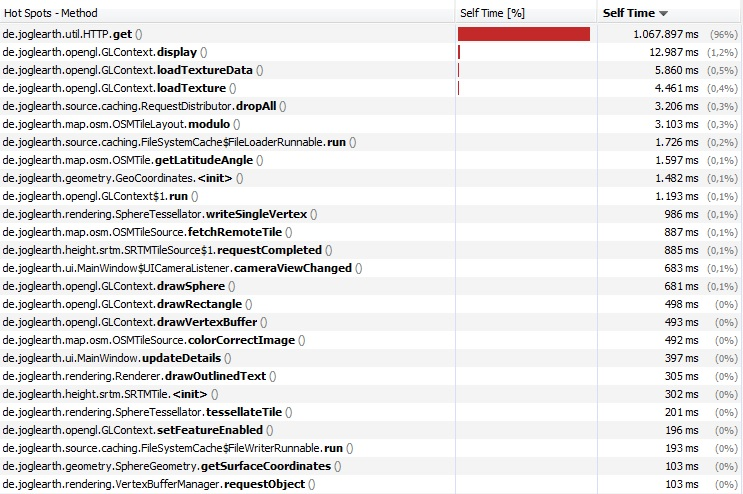
\includegraphics[scale=0.8]{cpu_profiling_normal.jpg}
\end{figure}
\vspace{3mm}
Beim CPU-Profiling wurden die Erwartungen bestätigt, dass die meiste Zeit mit Laden von Daten aus dem Netz verwendet wird.
Zudem befanden sich auch andere Funktionen deren Zeitlast abzusehen war unter den Methoden mit dem höchsten Zeitverbrauch. Hier fielen uns keine Methoden auf deren Zeitverbrauch ungewöhnlich war.
\newpage
\section{Speicher-Profiling}
\begin{figure}[!htb]
\centering
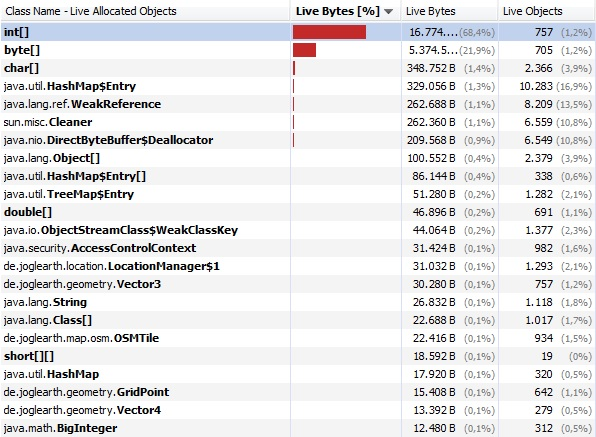
\includegraphics[scale=0.8]{memory_profile_normal.jpg}
\caption{Normaler Programmablauf}
\end{figure}
\begin{figure}[!htb]
\centering
\hspace{5mm}
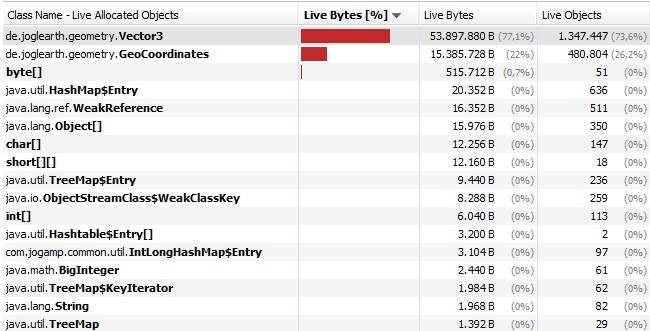
\includegraphics[scale=0.8]{memory_profile_shitgotreal.jpg}
\caption{Massenhaftes Auftreten von Vector3 Objekten}
\end{figure}
Das Speicher-Profiling verhielt sich im allgemeinen auch wie erwartet, die hohe Anzahl an ints entsteht durch die gespeicherten VertexBuffer und Texturen.
Bei einem Weiteren Profilingvorgang trat auf einmal ein rasanter Anstieg an Speicherverbrauch durch Vector3 Objecte hervor, dieser Bug wurde behoben.
\chapter{Änderungen zur Implementierung}
\section{Neue Klassen}
de.joglearth.geometry.TransformedTile\\
de.joglearth.opengl.TransformedTexture\\
de.joglearth.geometry.MapProjection\\
de.joglearth.geometry.LinearProjection\\
de.joglearth.geometry.MercatorProjection\\
de.joglearth.geometry.ProjectedTile\\
\section{Neue Methoden}
geometry.Tile.getScaledAlternative()\\
de.joglearth.map.osm.OSMTile.getScaledAlternative()\\
de.joglearth.map.single.SingleTile.getScaledAlternative()\\
de.joglearth.async.Invoker.canInvokeDirectly()\\
de.joglearth.geometry.Geometry.getLongitudeDisortion()\\
de.joglearth.geometry.PlaneGeometry.getLongitudeDisortion()\\
de.joglearth.geometry.SphereGeometry.getLongitudeDisortion()\\
de.joglearth.geometry.Geometry.allowsLongitudalTraversal()\\
de.joglearth.geometry.PlaneGeometry.allowsLongitudalTraversal()\\
de.joglearth.geometry.SphereGeometry.allowsLongitudalTraversal()\\
de.joglearth.geometry.location.LocationManager.enableLocations()\\
\section{Geänderte Signaturen}
de.joglearth.rendering.TextureManager.getTexture()\\
de.joglearth.rendering.Tessellator.tessellateTile()\\
de.joglearth.rendering.PlaneTessellator.tessellateTile()\\
de.joglearth.rendering.SphereTessellator.tessellateTile()\\
de.joglearth.async.AbstractInvoker.canInvokeDirectly()\\
de.joglearth.opengl.GLContext.canInvokeDirectly()\\
de.joglearth.async.AWTInvoker.canInvokeDirectly()\\
de.joglearth.geometry.location.LocationManager.getDetails()\\


\chapter{Lines of Code}
Zu Ende von Milestone 3:
\begin{longtable}{|l|p{3,6cm}|p{3,6cm}|p{3,6cm}|}
\hline
Phase & Code & Kommentare & Leere Zeilen\\
\hline
\hline
Implementierungs-Phase & 11088 & 3180 & 2861 \\
\hline
Validierungs-Phase & 12569 & 3325 & 2971 \\
\hline
\end{longtable}
\vspace{3mm}

Seit Ende von Milestone 3 haben sich geändert:
\begin{longtable}{|p{4,8cm}|p{4,9cm}|p{4,9cm}|}
\hline
Dateien & Hinzugefügte Zeilen & Gelöschte Zeilen \\
\hline
\hline
264 & 47309 & 8864 \\
\hline
\end{longtable}

\end{document}
